\begin{figure}[H]
    \centering
    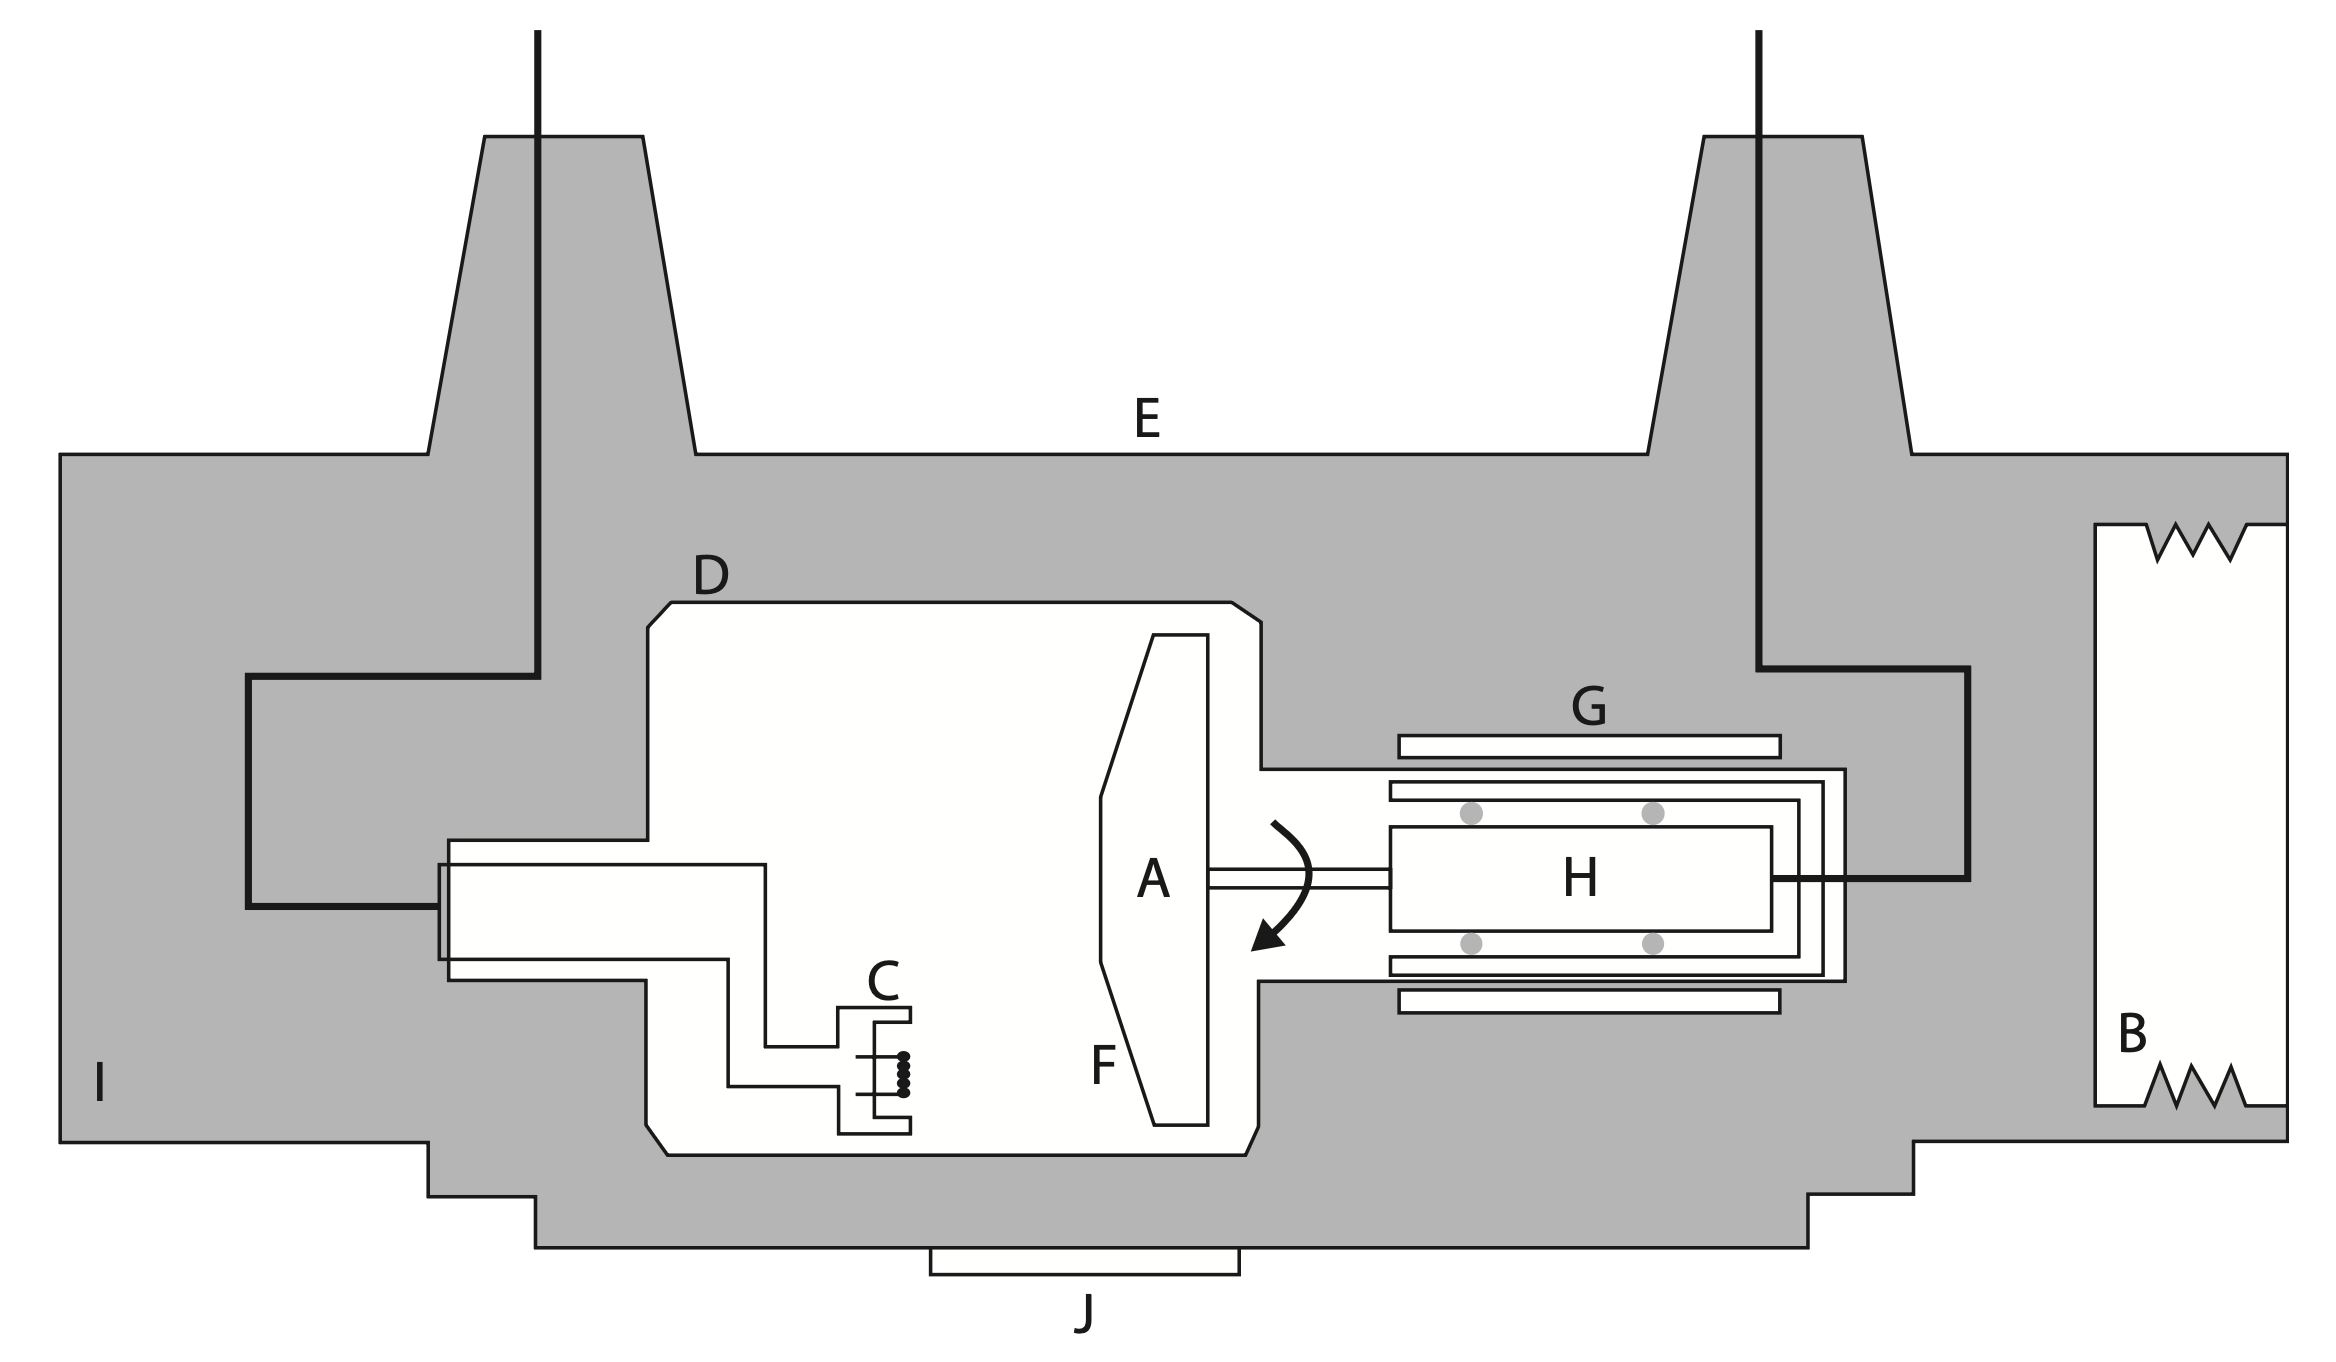
\includegraphics[width=0.9\textwidth]{Figures/Theory_Figures/X-ray tube.png}
    \caption{X-ray tube schematic diagram. A: Anode target, B: Bearing, C: Cathode filament, D: Envelope, E: Housing, F: Target, G: Stator, H: Rotor, I: Oil, J: Window \cite{Ng2022Set}}
\end{figure}

\subsection{X-ray tube exposure parameter affect the output}
\begin{enumerate}
    \item Tube voltage (kV): Changing tube voltage changes the total number of photons emitted (quantity) and the photon energies (quality). This is because although the number of bombarding electrons is the same, theprobability of X-ray production increases with increased tube voltage. Increasing the kV may result in the appearance of more characteristic X-ray photons and the shifting of the mean photon energy to higher energy (keV) (see Figure ). The relationship between the X-ray outputs with tube voltage is often approximated as follows: \[\text{Output} \propto \text{kV}^2\]
    \item Tube current (mA): Increasing the tube current results in an increase of the amount of electrons used to produce X-rays (Figure ). Thus, there is an increase in the quantity of the electrons as well as the X-ray photons produced. The X-ray quality remains essentially the same, i.e. the maximum photon energy and the effective photon energy remains unchanged. \[\text{Output} \propto \text{mA}\]
    \item Time of exposure (s): Time of exposure determines the number of electrons striking theanode. The number of X-ray photon increases with longer exposure time. \[\text{Output} \propto \text{exposure time}\]
    \item Filtration: Filtration changes the quantity and quality of the X-ray tube output. Filtration can be due to inherent filters such as oil and the window of the tube housing. Filtration can also be due to additional filters placed in the beam path. With increased filtration, the number of X-ray photons is reduced and the mean energy of the X-ray energy spectrum shifts to a higher energy (Figure ). This is because a proportion of the low energy photons is attenuated or filtered. K-edge filters are special filters that behave as a bandpass filter to allow the transmission of X-ray photons of a certain energy window.
    \item Target material: The probability of X-ray production, or X-ray yield, increases with the use of X-ray targets made of high atomic number (Z) materials (Figure ). X-ray output generally increases in the total number of photons produced. Characteristic X-ray photons with higher energies are also produced using a target material with higher Z.
\end{enumerate}

% 4 images side by side using minipage
\begin{figure}[H]
    \centering
    \begin{minipage}{0.24\textwidth}
        \centering
        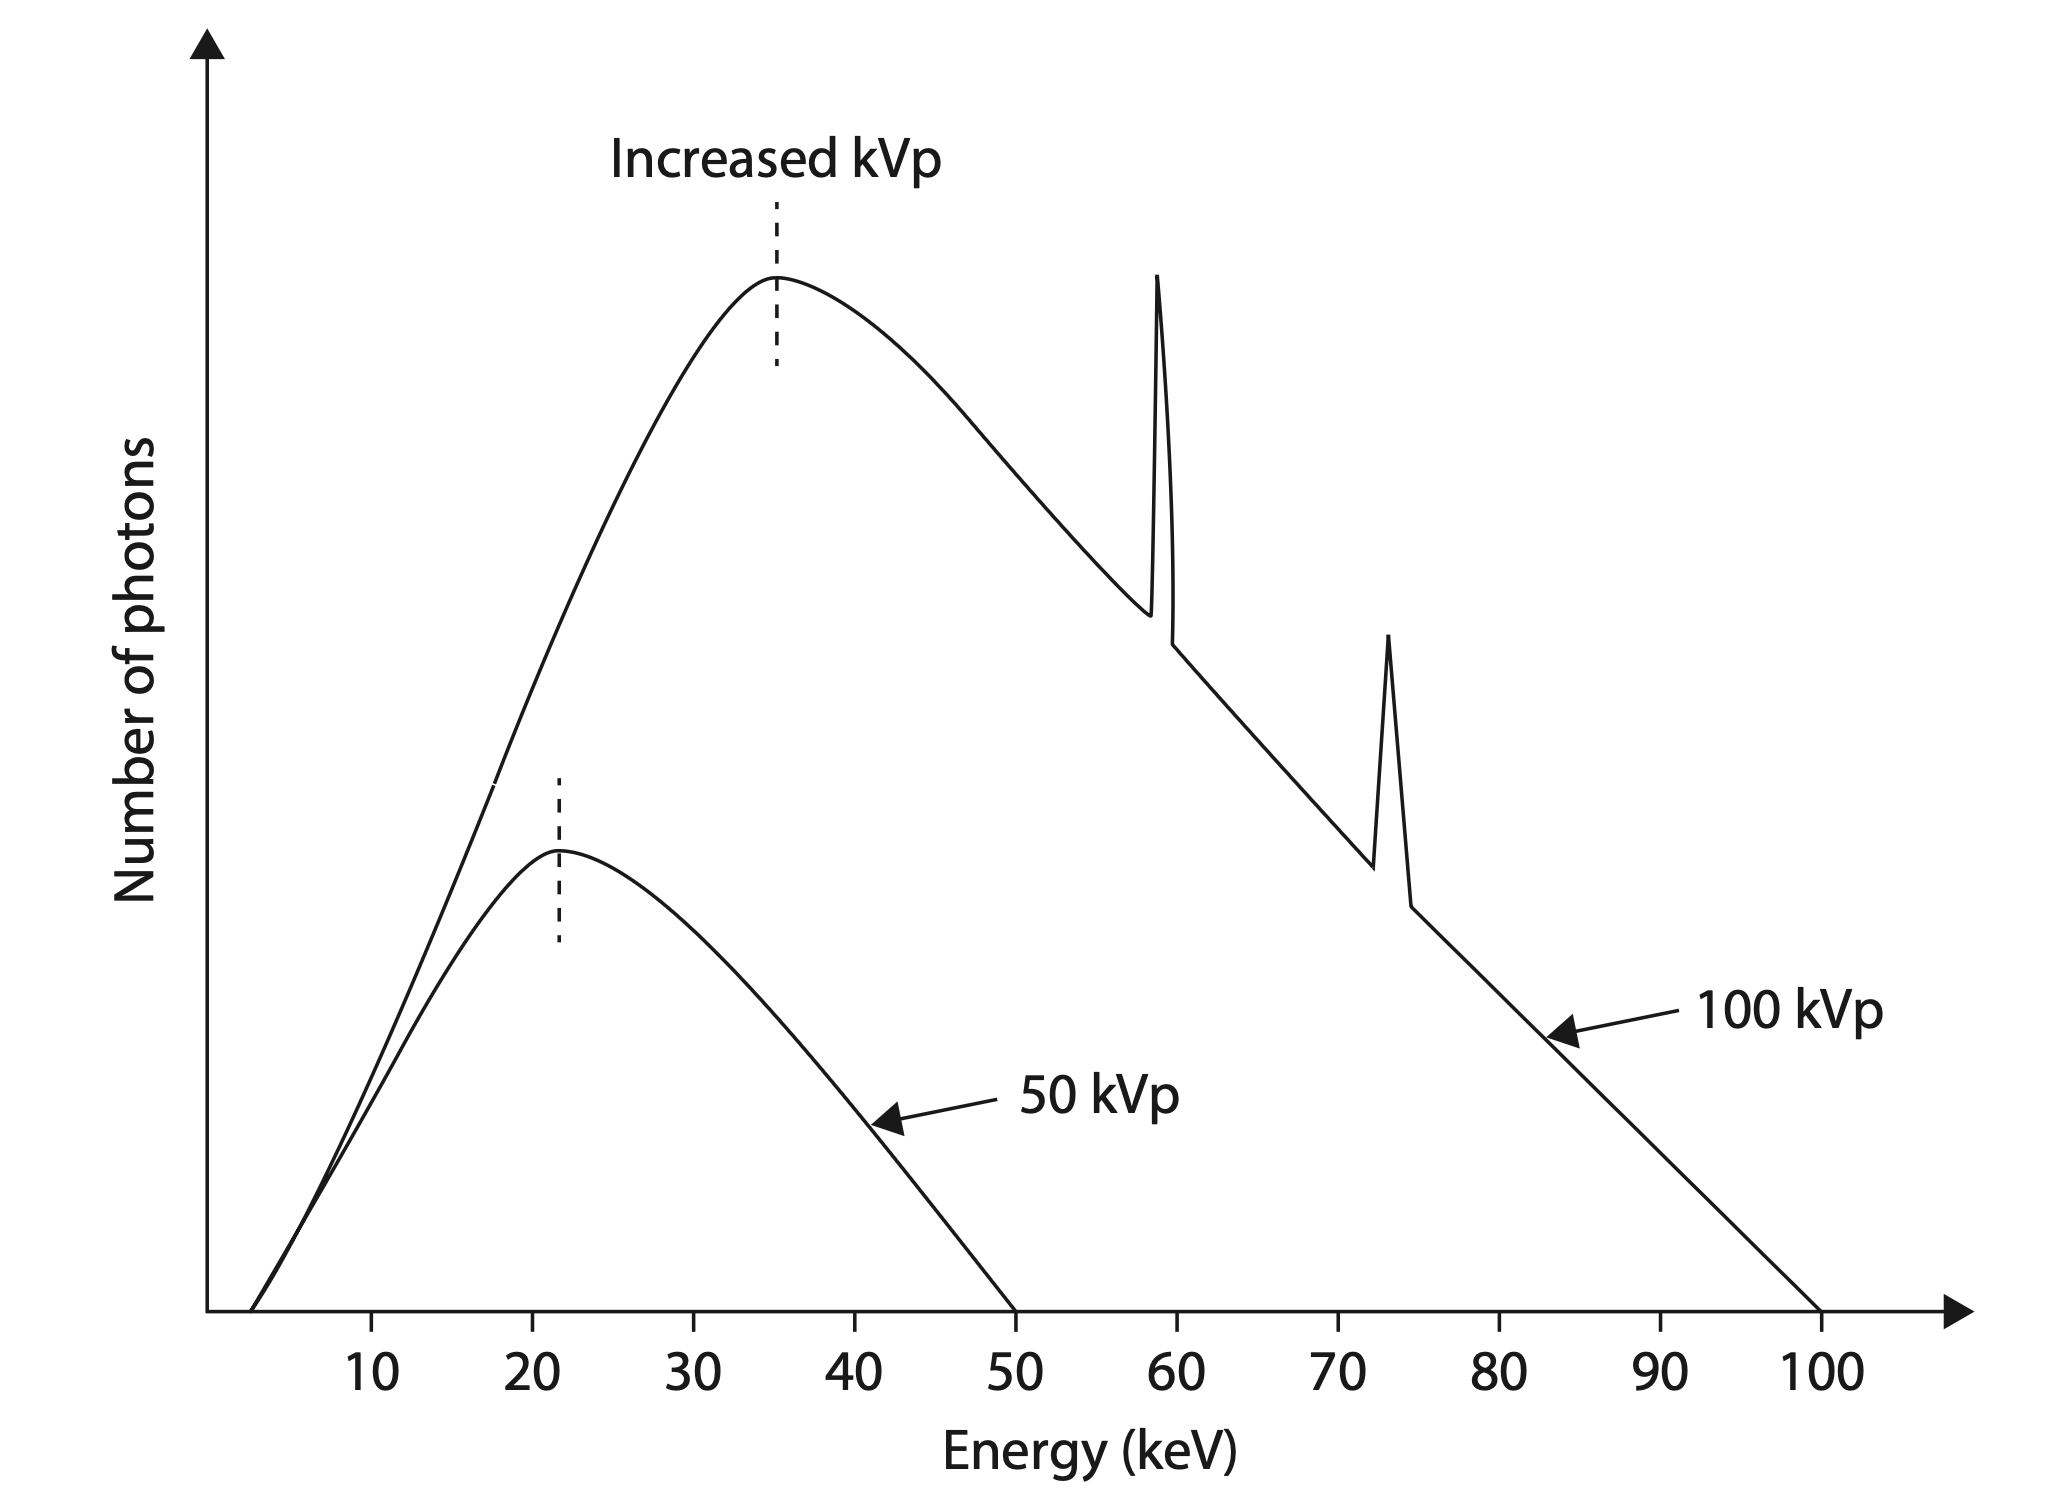
\includegraphics[width=\textwidth]{Figures/Theory_Figures/Tube Voltage vs Output.png}
        \caption{Tube Voltage vs Output}
        \label{}
    \end{minipage}\hfill
    \begin{minipage}{0.24\textwidth}
        \centering
        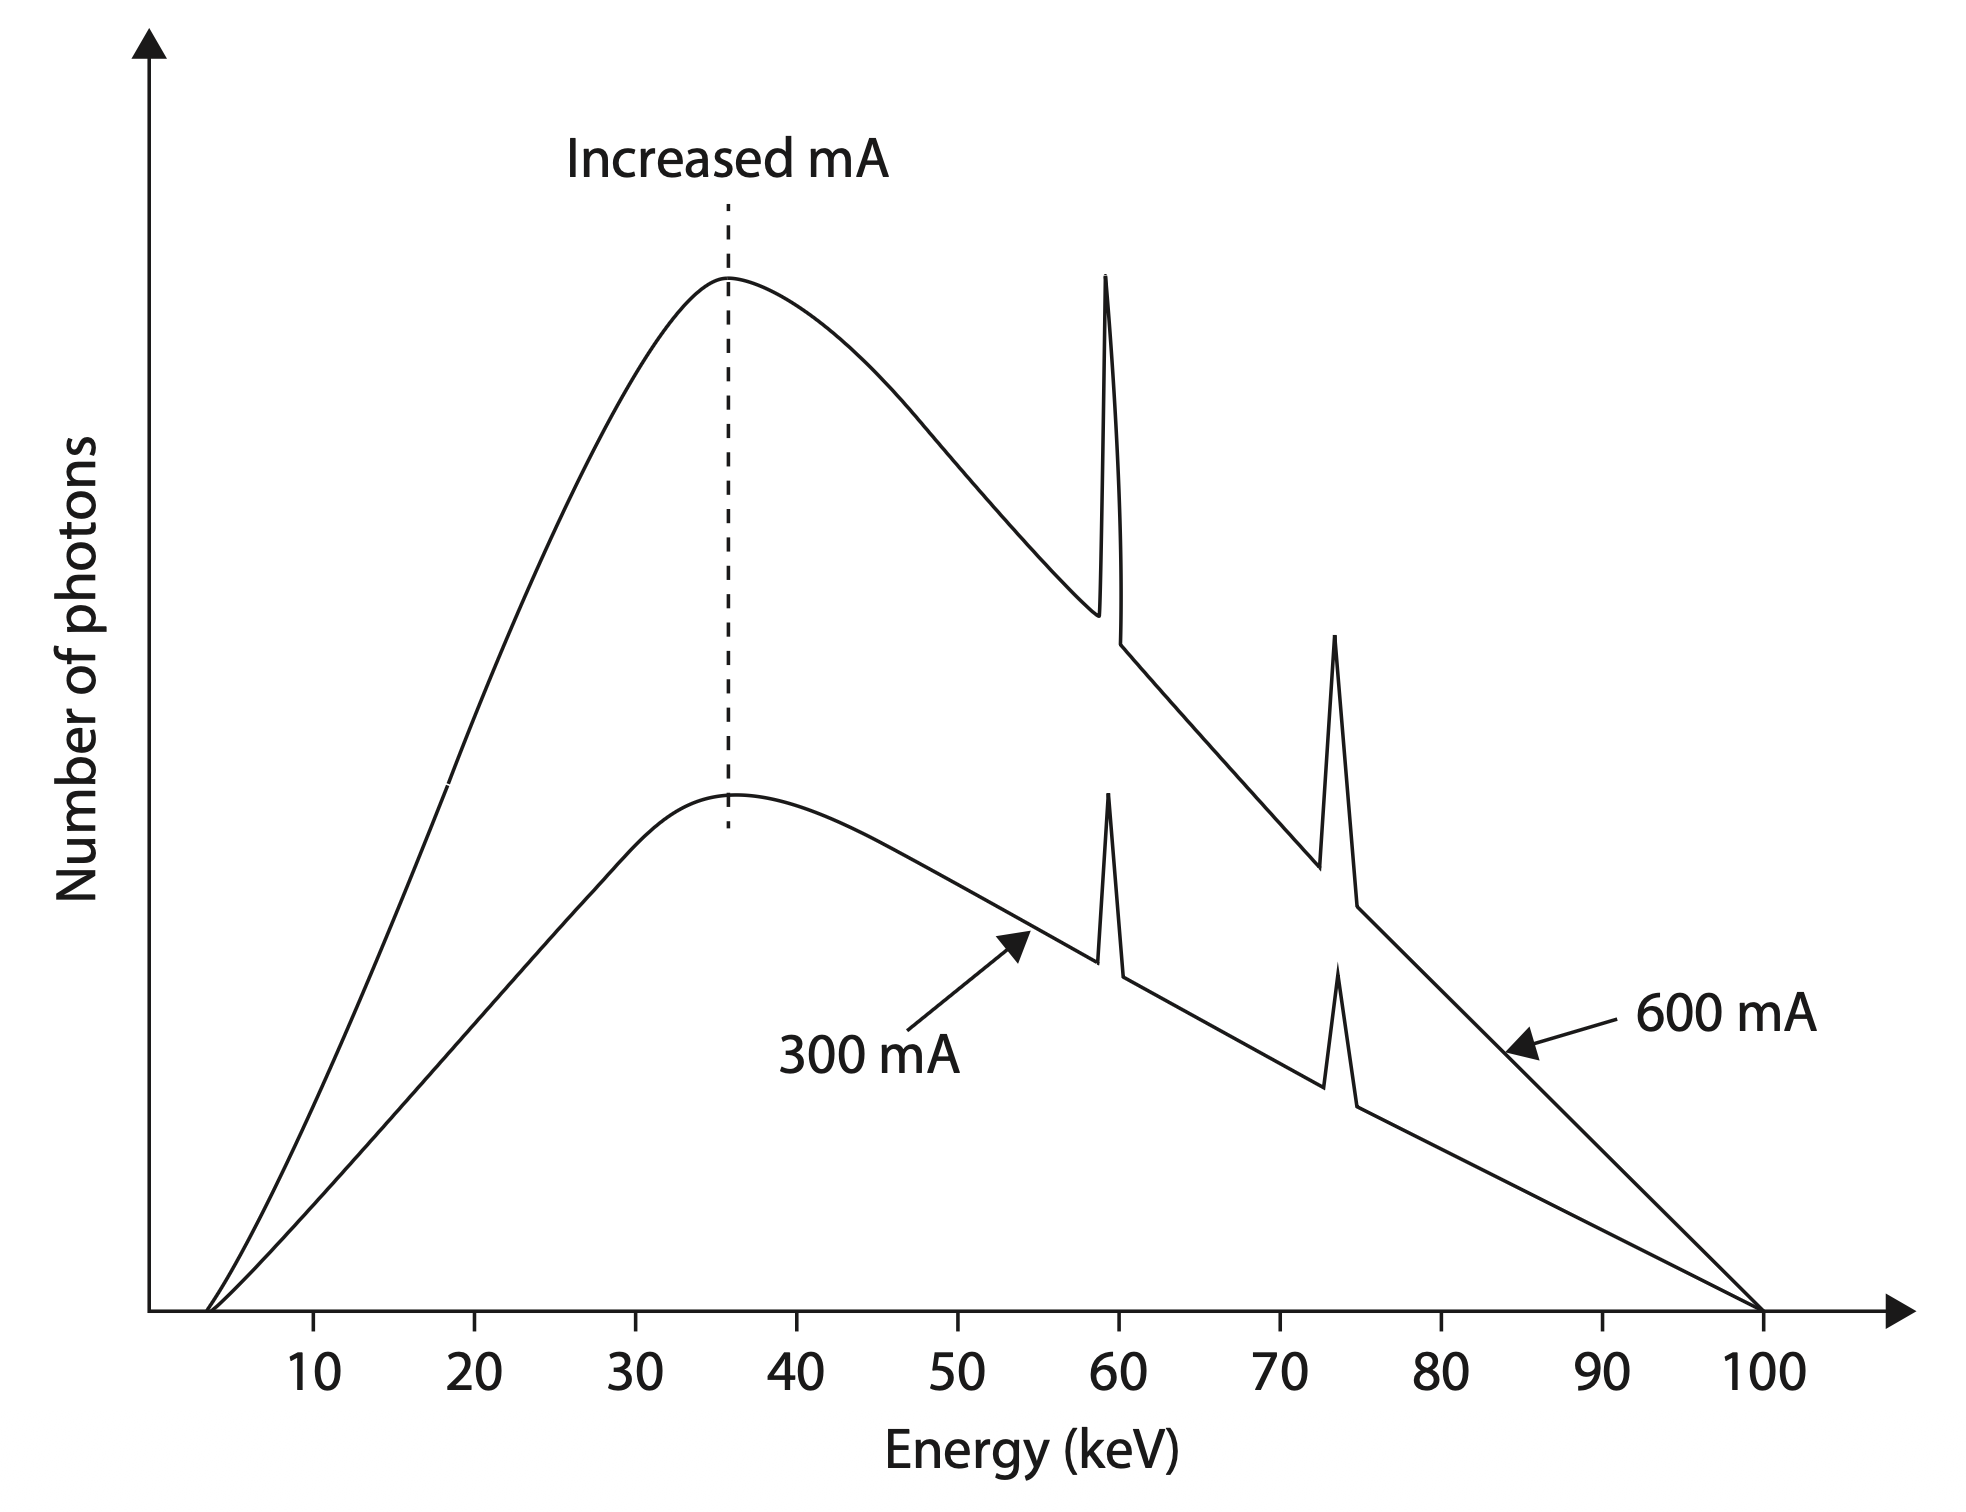
\includegraphics[width=\textwidth]{Figures/Theory_Figures/Tube Current vs Output.png}
        \caption{Tube Current vs Output}
        \label{}
    \end{minipage}\hfill
    \begin{minipage}{0.24\textwidth}
        \centering
        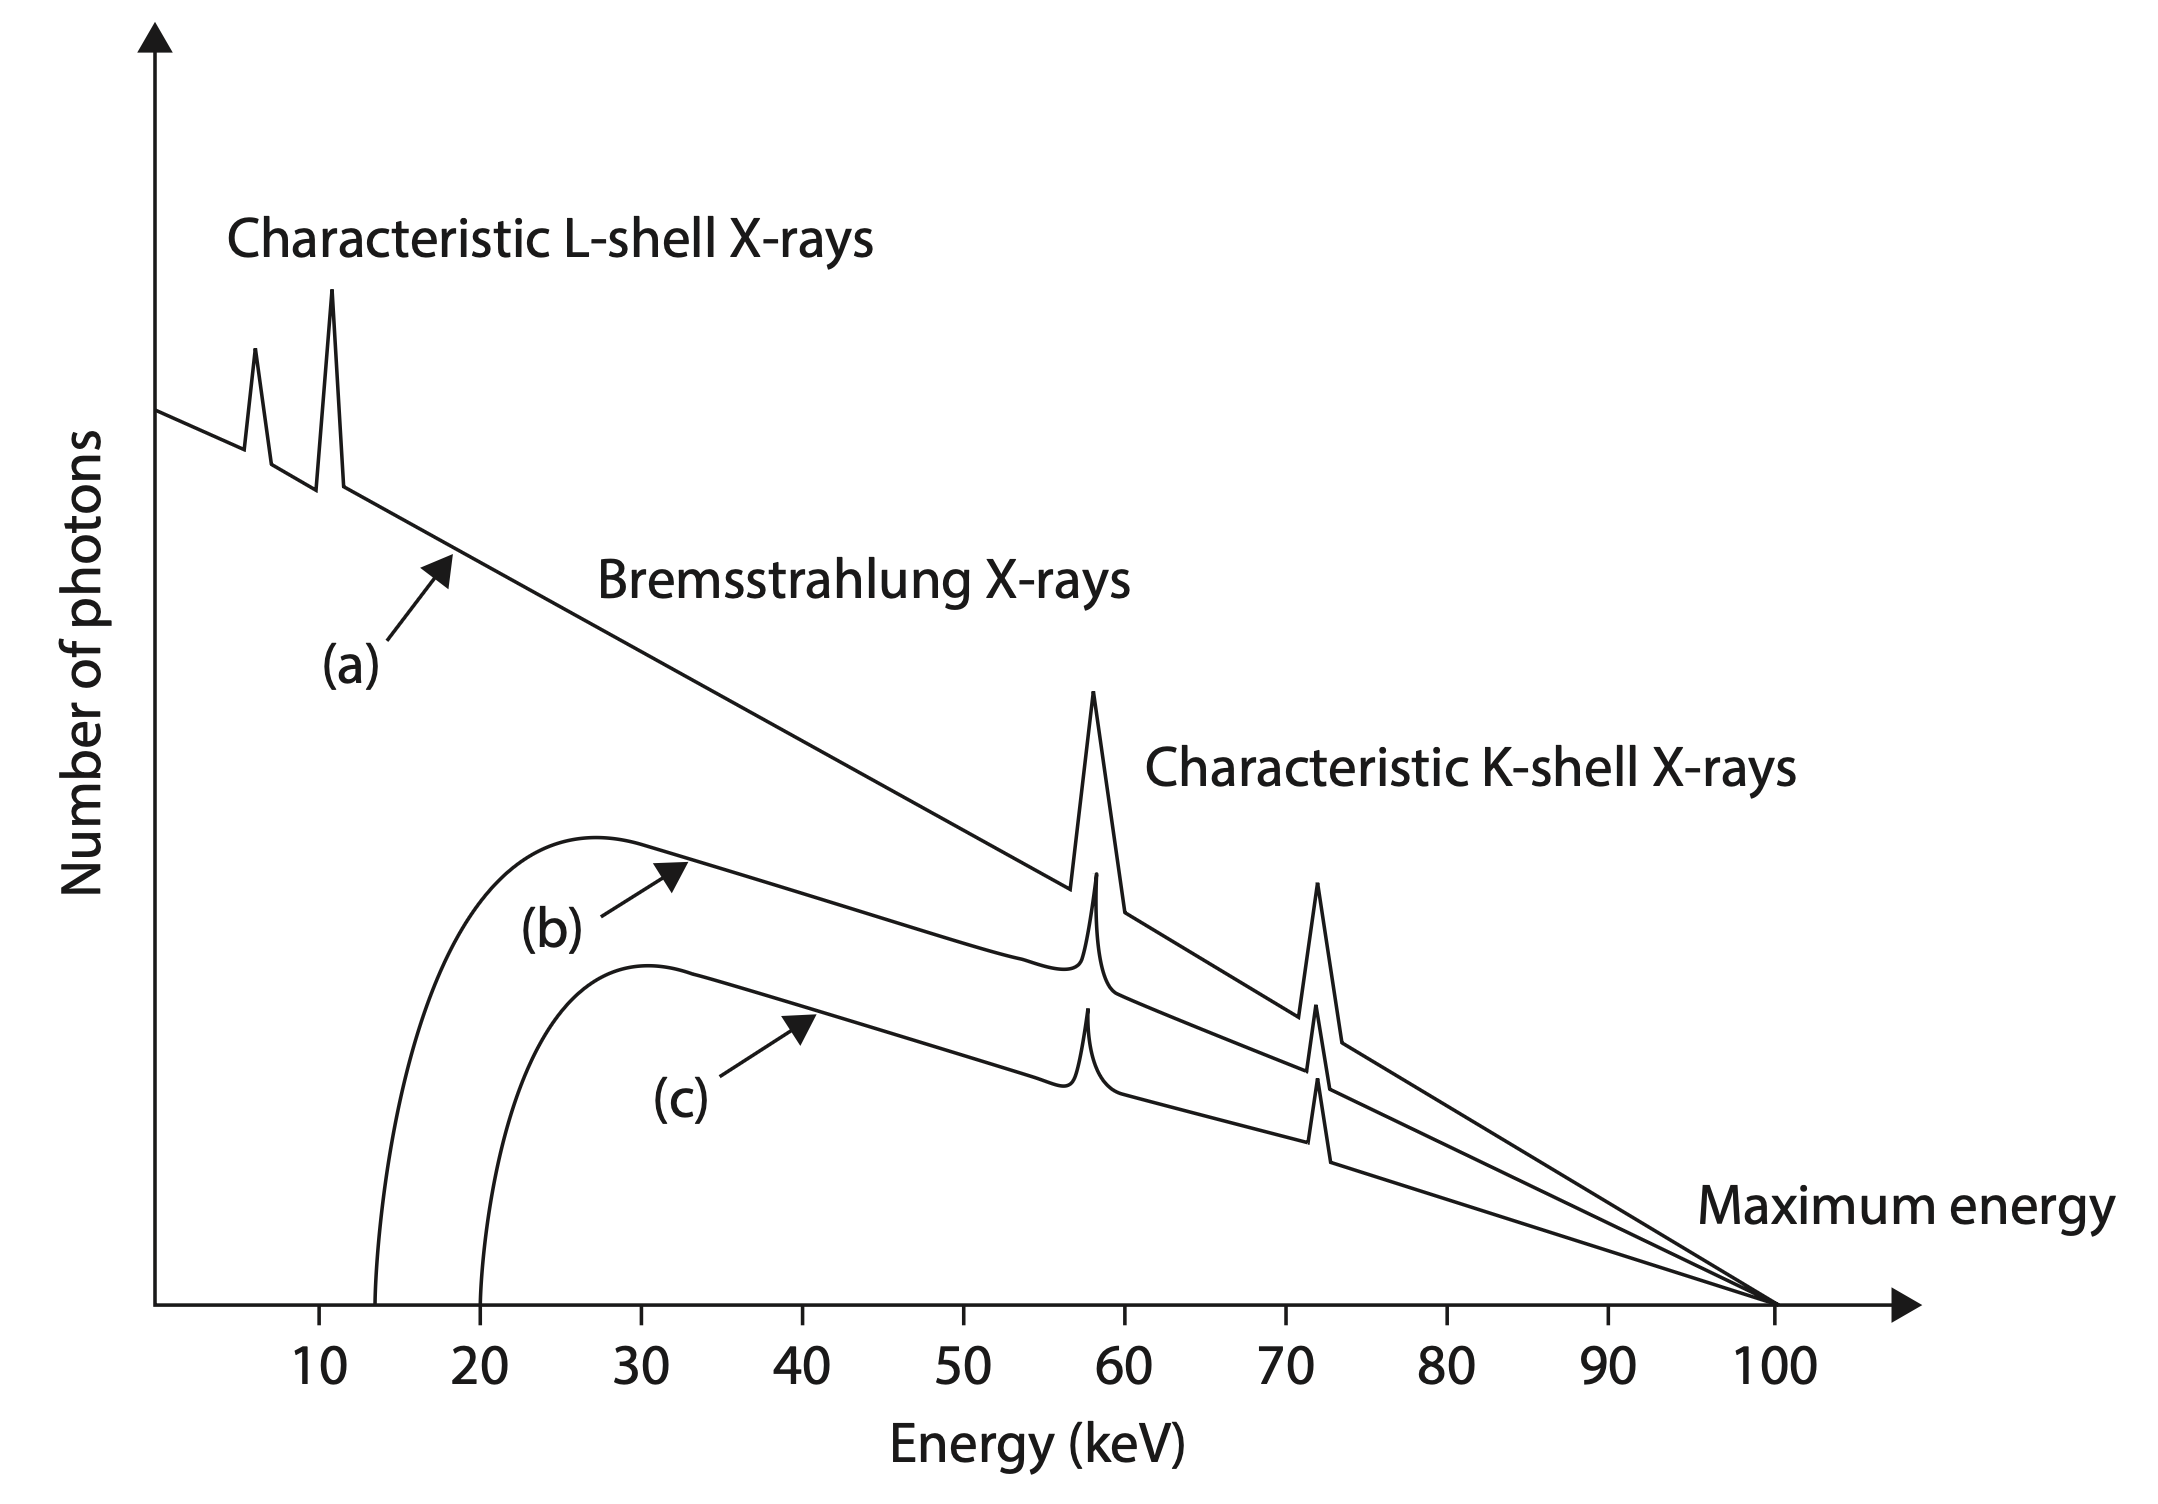
\includegraphics[width=\textwidth]{Figures/Theory_Figures/Filtration vs Output.png}
        \caption{Filtration vs Output}
        \label{}
    \end{minipage}\hfill
    \begin{minipage}{0.24\textwidth}
        \centering
        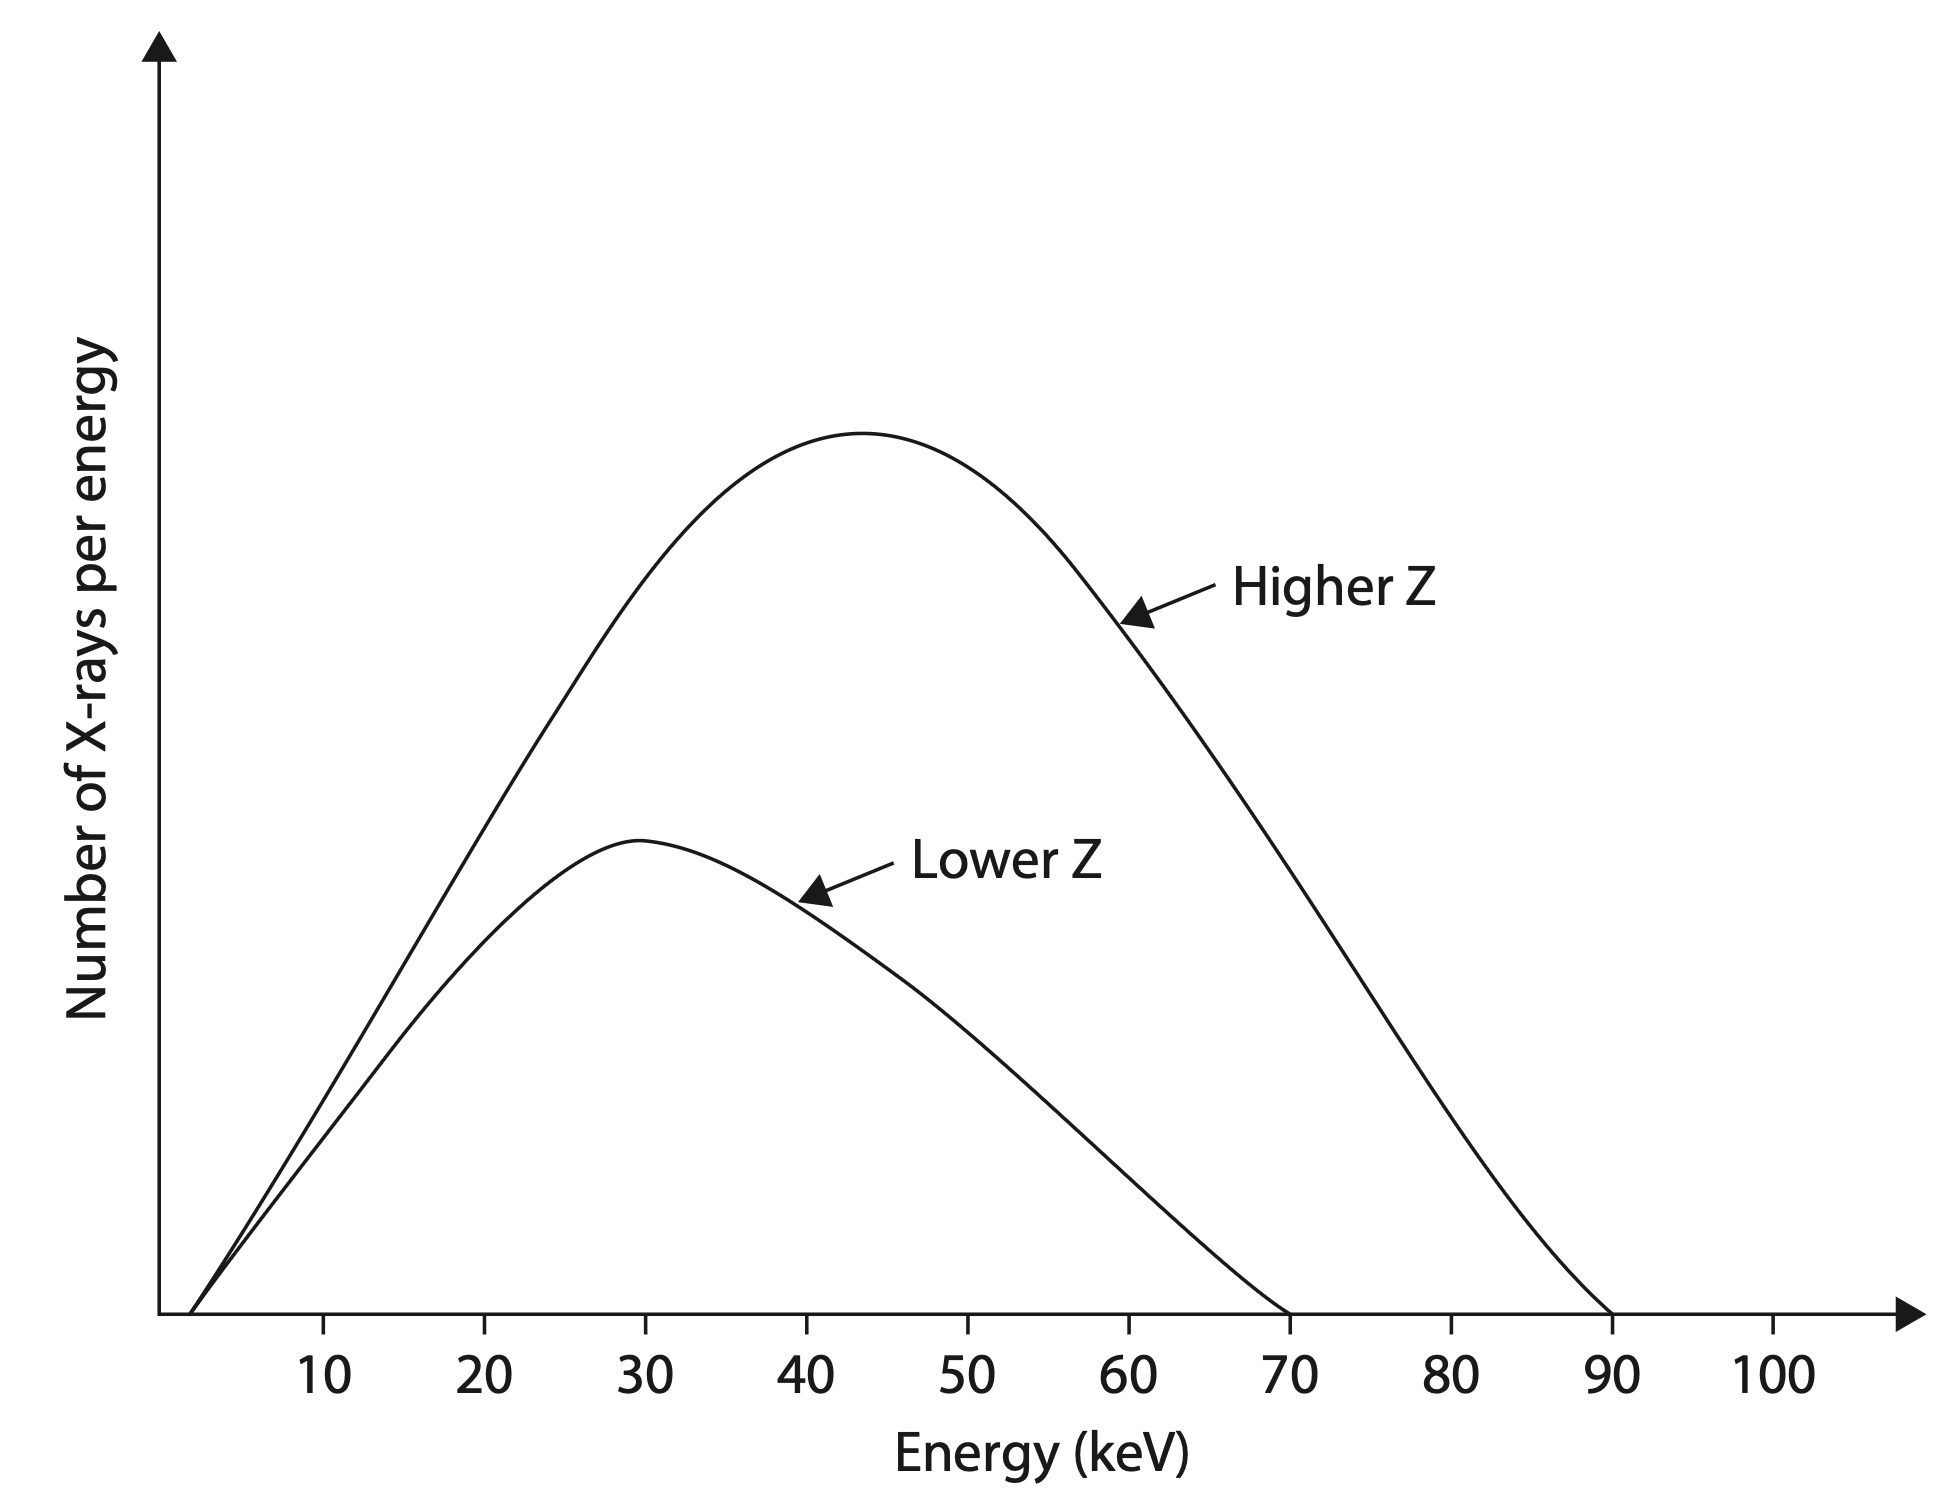
\includegraphics[width=\textwidth]{Figures/Theory_Figures/Target Material vs Output.png}
        \caption{Target Material vs Output}
        \label{}
    \end{minipage}
\end{figure}


The Quality assurance (QA) of diagnostic X-ray machines is a critical aspect of medical physics that ensures the safety, reliability, and optimal performance of these imaging devices. Regular QA procedures help in maintaining image quality, minimizing radiation exposure to patients and staff, and ensuring compliance with regulatory standards. Diagnostic X-ray machines are widely used in medical imaging for various applications, including radiography, fluoroscopy, and computed tomography (CT). The QA process involves a series of tests and evaluations designed to assess the performance of the X-ray equipment and its components. These tests typically include assessments of image quality parameters such as spatial resolution, contrast resolution, noise levels, and uniformity. Additionally, QA procedures evaluate the accuracy of radiation dose delivery, beam alignment, and mechanical integrity of the equipment. Regular QA checks are essential to identify any deviations from established performance standards, which may arise due to equipment wear and tear, calibration drift, or other factors. By promptly addressing these issues, healthcare facilities can ensure that diagnostic X-ray machines operate within acceptable limits, thereby enhancing patient safety and diagnostic accuracy.
The responsibility of quality control rests upon the Medical Physicist and the Technical staff of the diagnostic department. The test procedure involves the following steps: Carry out the QA tests as per the prescribed procedures, Record the results, Analyze the results, Seek corrective and preventive measures if the results are not satisfactory, Repeat the tests until satisfactory results are obtained.

In QA tests, the accuracy and consistency of various parameters, which influence the quality of diagnostic images and patient dose, are checked. The procedure for each experiment is given below.
\begin{itemize}
    \item Congruence of optical and radiation fields
    \item Central beam alignment
    \item Focal spot size
    \item Exposure time
    \item Applied tube potential (kVp)
    \item Total filtration
    \item Linearity of mA loading stations
    \item Consistency of radiation output
    \item Radiation leakage through tube housing
    \item Measurement of Low \& High Contrast sensitivity
    \item Radiation protection survey
\end{itemize}

\subsection{Congruence of Optical and Radiation Fields}
The congruence of the optical and radiation fields is a crucial quality assurance test for diagnostic X-ray machines. This test ensures that the area indicated by the optical light field accurately represents the area exposed to X-rays during imaging. Proper alignment between these fields is essential for accurate patient positioning and optimal image quality, as any misalignment can lead to unintended radiation exposure to non-targeted areas and compromise diagnostic outcomes.

Place the phantom on the table, between the image detector and the X-ray tube in such a way that the phantom so its center and main axis align with the markers of the apparatus. Limit the light field to the chosen rectangular marking on the phantom surface. Make the exposure. Measure the distance between the light field borders and actual X-ray beam borders in perpendicular and parallel directions. Use a clearly marked scale on the phantom. The sum of differences between the light and the X-ray field in perpendicular and parallel directions should not be greater than 2\% of the FFD (Focal spot to Film distance).

\subsection{Central beam alignment}
The image may be distorted if the X-ray beam is not perpendicular to the image receptor (Detector). For this test, screw the optional cone on the phantom. The optional cone has a stainless- steel ball on the top and a circular steel patch at the bottom. Make the exposure. If the image of the ball lies entirely within the image of the circular patch, then the deviation of the beam from the tube axis is not more significant than $1.5^\circ$.
\subsection{Focal spot size}
The ability to resolve the smallest image size (i.e., Spatial Resolution) in a radiograph depends on the focal spot size. Since the focal spot size may be altered due to the bombardment of electrons with the target, it must be checked periodically to ensure that it is within acceptable limits. Focal spot size is evaluated on the principle of minimum resolution and a Bar/hole test pattern is employed for evaluating focal spot size. At minimum resolution, the edge gradient (penumbra) of one pattern of the pair merges with the image of the other, and the images of both patterns of the pair cannot be resolved separately. When this happens, focal spot size (f), line width, and Magnification (M) are related as follows: 
\[f = \frac{M}{M-1} \times \text{Line width}\]
Where, M = Source-to-film distance / Source-to-pattern distance

To perform this test, a resolution bar pattern is mounted on the phantom such that the source- to-pattern distance is three times the pattern-to-film/detector distance. The resolution bar pattern consists of several groups of lines (slits) of sizes gradually decreasing in dimension. Expose the bar pattern. Perform two measurements in two bar pattern positions: parallel and perpendicular to the bottom edge of the phantom. A given pattern must be resolved in both directions to count. From the resolved Line Width, the focal spot size can be calculated using the above formula.
\subsection{Exposure time}
The accuracy of the exposure time is essential for obtaining consistent image quality and controlling patient dose. If the exposure time of the X-ray diagnostic unit is not in order, the radiograph can be underexposed or overexposed. There may be a change in the adequate tissue contrast resolution in the image. The Cobia Smart R/F detector can measure the exposure time.

\subsection{Applied tube potential (kVp)}
The applied kilovoltage affects the quality and quantity of X-rays reaching the image receptor (Detector) and hence the contrast and density of the radiograph. Since any variation from the set kVp can affect the quality of the radiograph, the kVp settings must be checked periodically. kVp can be measured by the Cobia Smart R/F.

\subsection{Total filtration}
A specific minimum filtration must be present in the X-ray tube to cut off low-energy components from the X-ray beam. These low-energy components do not contribute to image formation but result in unnecessary patient exposure. If the filtration is too high, the attenuation will be more and image contrast will be reduced. Therefore, the total filtration for the X-ray tube should be optimum for patient safety and image quality. For this purpose, regulatory bodies (AERB) recommend total filtration for X-Ray machines for different maximum-rated tube potentials. Total filtration includes inherent filtration and added filtration. Hence total filtration evaluation is necessary to verify whether the added filtration is adequate. If not adequate, additional filtration must be provided for the x-ray tube. The Cobia Smart R/F detector can measure the total filtration.

\subsection{Linearity of the mA loading station}
Keeping the kVp and time constant, the radiation output is measured at different mA stations.
Measurement for each mA station is to be repeated for several times to eliminate statistical errors.
Each mA station reading is averaged, and the coefficient of linearity (COL) is evaluated from average
mR/ mAs or mGy/ mAs (X) as follows. The tolerance is 0.1.
\[ \text{Coefficient of Linearity}= \frac{x_{max} - x_{min}}{x_{max} + x_{min}}\]

\subsection{Consistency (reproducibility) of radiation output}
Keeping fixed mA and time, radiation output is measured at various available kVp stations. The
average of mR/mAs (mGy/mAs) is calculated (X). Consistency at each kVp station is checked by
evaluating the Coefficient of Variation (COV). The COV should not exceed 0.05.
\[COV = \frac{1}{X}\sqrt{\frac{(X_i - X)^2}{n-1}}\]
Where, Xi = individual reading, n = number of readings


\subsection{Radiation leakage through tube housing}
As per AERB Safety Code on Diagnostic X-ray Equipment and installations, every housing for
medical diagnostic X-ray equipment shall be so constructed that the leakage radiation through the
protective tube housing in any direction shall not exceed an air kerma of 1.0mGy (about 114mR) in
one hour at 1.0m from the x-ray target. The measurement conditions are given below.
\begin{itemize}
    \item Averaged over an area not larger than 100 cm$^2$
    \item No linear dimension greater than 20cm
    \item Operating at maximum rated kVp and for the maximum rated current at that kVp.
\end{itemize}

The radiation leakage measurement is carried out with an ionization radiation survey meter. For checking the leakage radiation, the collimator of the tube housing is fully closed. The operating time should be greater than the time constant of the survey meter. The exposure rate at one meter from the target is measured at different locations (anode side, cathode side, front back, and top) from the tube housing and collimator. For the maximum leakage rate (mR/h) for both tube housing and collimator, leakage in one hour is computed based on the workload of the machine. 180mA-min in one hour is taken as the maximum workload of a diagnostic machine.
Hence leakage in one hour will be:
\[\text{Leakage in one hour (mR)} = \text{Leakage rate (mR/h)} \times \frac{180}{\text{Operating mA-min}}\]
\subsection{Measurement of Low \& High Contrast sensitivity}
Low contrast sensitivity refers to the ability of a system to visualize low-contrast objects or structures. In clinical practice, patient diagnoses are frequently made on the perception of the fluoroscopic image of small low-contrast anatomic structures. The number of visible low-contrast objects should not change over time.

The high contrast sensitivity allows for a simple evaluation of system resolution to ensure that optimal anatomic detail is visible to the practitioner. High contrast resolution is essential for all fluoroscopic procedures. Using the zoom tool, assess the Line Pairs per millimeter resolution. It is the highest number next to the group of lines where three separate lines can be distinguished.

\subsection{Radiation protection survey}
A radiation protection survey is a series of measurements of radiation levels at various locations around the diagnostic X-Ray machine installation. This is done to check whether the radiation levels around the building are within the permissible limits as mandated by the Competent Authority (AERB). A pressurized ion chamber-based survey meter is used to measure the radiation levels.